\documentclass[a4paper]{article}
\usepackage[fontsize=9.4pt]{scrextend}

% --- Packages for LuaLaTeX (Multilingual: English + Vietnamese + Classical Chinese) ---
\usepackage{fontspec}
\directlua{
  luaotfload.add_fallback("cjkfallback", {
    "file:msjh.ttc:index=0;mode=node;",
    "file:mingliub.ttc:index=0;mode=node;",
    "file:simsun.ttc:index=0;mode=node;",
    "file:simsunb.ttf:mode=node;"
  })
}
% Enable natural line-breaking between CJK characters in LuaLaTeX (built-in luatexbase)
\directlua{
  local glyph_id = node.id("glyph")
  local glue_id  = node.id("glue")
  local function is_cjk(c)
    return (c >= 0x3000 and c <= 0x303F)
        or (c >= 0x3400 and c <= 0x9FFF)
        or (c >= 0xF900 and c <= 0xFAFF)
        or (c >= 0xFF00 and c <= 0xFFEF)
  end
  local function add_cjk_breakable_glue(head)
    local cur = head
    while cur do
      if cur.id == glyph_id and cur.next and cur.next.id == glyph_id then
        if is_cjk(cur.char) or is_cjk(cur.next.char) then
          local g = node.new(glue_id)
          node.setglue(g, 0, 12000, 0, 0, 0)
          head = node.insert_after(head, cur, g)
          cur = g
        end
      end
      cur = cur.next
    end
    return head
  end
  luatexbase.add_to_callback("pre_linebreak_filter", add_cjk_breakable_glue, "cjk_break")
}

\usepackage[margin=1.28cm, top=1.18cm, bottom=1.22cm]{geometry}
\usepackage{amsmath,amssymb}
\usepackage{graphicx}
\usepackage{booktabs}
\usepackage{tabularx}
\usepackage{multirow}
\usepackage{array}
\usepackage{enumitem}
\usepackage{xcolor}
\usepackage{tikz}
\usetikzlibrary{shapes.geometric, arrows.meta, positioning, calc, backgrounds, fit}
\usepackage{titlesec}
\usepackage{needspace}
\usepackage{caption}
\usepackage[colorlinks=true, linkcolor=blue!65!black, urlcolor=blue!65!black, citecolor=blue!65!black]{hyperref}

% --- Fonts (Resolved via OSFONTDIR -> Instant Load, Full Viet + CJK) ---
\setmainfont{times.ttf}[
  BoldFont = timesbd.ttf,
  ItalicFont = timesi.ttf,
  BoldItalicFont = timesbi.ttf,
  RawFeature = {fallback=cjkfallback}
]
\setsansfont{arial.ttf}[
  BoldFont = arialbd.ttf,
  ItalicFont = ariali.ttf,
  BoldItalicFont = arialbi.ttf,
  RawFeature = {fallback=cjkfallback}
]
\setmonofont{consola.ttf}[
  Scale = 0.84,
  BoldFont = consolab.ttf,
  ItalicFont = consolai.ttf,
  BoldItalicFont = consolaz.ttf,
  RawFeature = {fallback=cjkfallback}
]

% --- Color Palette ---
\definecolor{primary}{HTML}{1B4F72}
\definecolor{secondary}{HTML}{2874A6}
\definecolor{accent}{HTML}{C0392B}
\definecolor{softbg}{HTML}{F4F7FA}
\definecolor{bordercol}{HTML}{BDD0E0}
\definecolor{okgreen}{HTML}{1E8449}
\definecolor{warnamber}{HTML}{D68910}

% --- Compact Academic Spacing (< 5 Pages Target: 4 Full Balanced Pages) ---
\setlength{\parindent}{0pt}
\setlength{\parskip}{2.6pt}
\emergencystretch=1.6em
\setlist[itemize]{leftmargin=1.30em, itemsep=1.1pt, topsep=1.1pt, parsep=0pt}
\setlist[enumerate]{leftmargin=1.45em, itemsep=1.2pt, topsep=1.2pt, parsep=0pt}
\captionsetup{font={footnotesize}, labelfont={bf,color=primary}, skip=2.2pt}

\titleformat{\section}{\normalsize\large\bfseries\color{primary}}{\thesection.}{0.42em}{}[\vspace{-3pt}\textcolor{bordercol}{\titlerule[0.8pt]}]
\titlespacing*{\section}{0pt}{5.5pt}{3pt}
\titleformat{\subsection}{\normalsize\bfseries\color{secondary}}{\thesubsection}{0.42em}{}
\titlespacing*{\subsection}{0pt}{4pt}{1.8pt}

\newcolumntype{Y}{>{\raggedright\arraybackslash}X}
\newcolumntype{L}[1]{>{\raggedright\arraybackslash}p{#1}}
\newcolumntype{C}[1]{>{\centering\arraybackslash}p{#1}}
\newcolumntype{R}[1]{>{\raggedleft\arraybackslash}p{#1}}

\begin{document}

% ==============================================================================
% HEADER BANNER
% ==============================================================================
\begin{tikzpicture}[remember picture, overlay]
  \fill[primary] ([yshift=-0.20cm]current page.north west) rectangle ([yshift=-0.35cm]current page.north east);
\end{tikzpicture}
\vspace{-0.45cm}
\begin{center}
  {\footnotesize\bfseries\sffamily\textcolor{secondary}{NATURAL LANGUAGE PROCESSING --- MIDTERM PROJECT REPORT (TOPIC CODE: CV16\_PhuBienTapLuc)}}\\[1.5pt]
  {\Large\bfseries\textcolor{primary}{Building a Classical Chinese--Vietnamese Parallel Corpus\\from Historical Scans of \textit{Phủ Biên Tạp Lục} (撫邊雜錄)}}\\[3pt]
  {\small \textbf{Student:} Trần Cảnh Anh Tuấn \quad|\quad \textbf{Student ID:} 24125048 \quad|\quad \textbf{Date:} November 2026}
\end{center}
\vspace{-6pt}
\noindent\textcolor{bordercol}{\rule{\textwidth}{0.6pt}}
\vspace{-7pt}

% ==============================================================================
% 1. INTRODUCTION
% ==============================================================================
\section{Introduction}
\textbf{Project Objective:} This project constructs a high-precision, sentence- and clause-level Classical Chinese--Vietnamese (\textit{Hán--Việt}) parallel corpus from historical scanned editions of \textit{Phủ Biên Tạp Lục} (撫邊雜錄, \textit{Miscellaneous Records of Pacifying the Frontier}, compiled by Lê Quý Đôn in 1776). Historical Sino-Vietnamese documents pose severe low-resource NLP challenges: Classical Chinese manuscripts lack punctuation, suffer from ink bleed and spine curvature, and read vertically right-to-left (RTL), while modern Vietnamese editions restructure syntax, attach dense footnotes, and interleave Sino-Vietnamese phonetic transcriptions (\textit{phiên âm}).

\textbf{Assigned Task \& Deliverable Compliance:} Executed individually under Topic \textbf{CV16}, the corpus spans two archival source groups partitioned into three genre-distinct blocks: \textbf{\texttt{Cap\_01}} (taxation registers, official stipends, and military boat quotas in Thuận Hóa \& Quảng Nam, 53 manuscript pages), \textbf{\texttt{Cap\_02\_V}} (Volume V: classical Tang-style poetry, prefaces, and diplomatic correspondence, 51 pages), and \textbf{\texttt{Cap\_02\_VI}} (Volume VI: regional geography and local products, 37 pages). Per \texttt{Guideline.pdf} for scanned PDF inputs requiring OCR, the mandatory individual benchmark is \textbf{$\ge$ 2,000 valid aligned pairs} with an alignment error rate strictly \textbf{$\le$ 30\%} (internal target $\le$ 20\%) across synchronized \texttt{CV16\_PhuBienTapLuc\_parallel.tsv} and \texttt{.xlsx} (\texttt{DONG\_HANG}) files, accompanied by cleaned \texttt{han.txt}/\texttt{viet.txt} files.

% ==============================================================================
% 2. DATA AND TOOLS USED
% ==============================================================================
\section{Data and Tools Used}
\subsection{Input Data Inventory and Structural Characteristics}
Prior to batch OCR, all source PDFs in \texttt{01\_nguon/} were audited in \texttt{Kiem\_ke\_nguon.xlsx} to establish content boundaries and cross-edition page anchors (Table~\ref{tab:inventory}). Notably, \texttt{Cap\_02/HAN.pdf} merges Volume V and Volume VI continuously (switching at page 51 via \texttt{撫邊雜錄卷之六}), whereas the Vietnamese scan splits them across separate intervals and places italic \textit{Phiên âm} verse blocks immediately above \textit{(Dịch):} translations in Volume V.

\begin{table}[!htb]
\centering
\caption{Source document inventory audited in \texttt{01\_nguon/Kiem\_ke\_nguon.xlsx}.}
\label{tab:inventory}
\scriptsize
\renewcommand{\arraystretch}{1.08}
\begin{tabularx}{\textwidth}{@{}l l l c L{3.35cm} Y@{}}
\toprule
\textbf{Block} & \textbf{Lang.} & \textbf{File (\texttt{01\_nguon/})} & \textbf{Pages (Content)} & \textbf{Archival Source} & \textbf{Format \& Physical Characteristics} \\
\midrule
\texttt{Cap\_01} & Hán & \texttt{Cap\_01/HAN.pdf} & 53 (52 unique) & Gallica BnF (\textit{Vietnamien A 18}) & PDF Scan; handwritten vertical RTL, dark spine shadow, page tilt, p.\,49 duplicated. \\
\texttt{Cap\_01} & Việt & \texttt{Cap\_01/VIET.pdf} & 251 (pp.\,186--251) & Published translation scan & PDF Scan with embedded OCR; noisy digits (\texttt{õ/ð}$\to$\texttt{5}, \texttt{I/l}$\to$\texttt{1}) and footnotes. \\
\texttt{Cap\_02} & Hán & \texttt{Cap\_02/HAN.pdf} & 92 (pp.\,1--87) & VNPF / NLV (\texttt{R.1606}) & PDF Scan; Vol.\,V (pp.\,1--51) \& Vol.\,VI (pp.\,51--87); pp.\,88--92 covers; spaced columns. \\
\texttt{Cap\_02} & Việt & \texttt{Cap\_02/VIET.pdf} & 105 + 36 & Reference scan (2007 ed.) & PDF Scan; Vol.\,V (pp.\,1--105, mixed \textit{Phiên âm} + verse) \& Vol.\,VI (pp.\,405--439). \\
\bottomrule
\end{tabularx}
\end{table}

\vspace{-3pt}
\subsection{Tools, Libraries, and Deep Learning Models}
\begin{itemize}
  \item \textbf{Geometry-Aware Image Pre-processing \& OCR (\texttt{02\_ocr\_tho}):} \texttt{PyMuPDF} (\texttt{144\,DPI}, $\le 2{,}000\text{\,px}$) \& \texttt{Poppler} (\texttt{pdftotext -layout} / \texttt{-bbox-layout}); \texttt{OpenCV} \& \texttt{SciPy} (\texttt{fastNlMeansDenoising}, \texttt{CLAHE}, \texttt{HoughLinesP}, \texttt{connectedComponentsWithStats}); \textbf{PaddleOCR GPU} (\texttt{lang='chinese\_cht'} on Kaggle Tesla T4) for vertical Traditional Chinese recognition.
  \item \textbf{Classical Segmentation \& Orthographic Restoration (\texttt{03\_text\_sach/v1--v4}):} \texttt{OpenCC} (\texttt{t2s} internal projection while preserving 100\% Traditional glyphs); HuggingFace token classifier \textbf{\texttt{guwen-biaodian}} (\texttt{raynardj/classical-chinese-punctuation-guwen-biaodian}); structural backward-lookahead \textit{Phiên âm} pruner and syllabic onset--nucleus--coda Vietnamese OCR spell-restorer.
  \item \textbf{Bilingual Alignment \& Blind Auditing (\texttt{04\_dong\_hang/v1--v6.2}):} Multilingual \textbf{LaBSE} (\texttt{sentence-transformers/LaBSE}), \textbf{Bertalign}, custom \textbf{Two-Pass Moore/Hunalign Anchor + Vecalign Overlap Aligner (\texttt{v5})}, \textbf{KimHanNom API} (HCMUS) + selective \texttt{CLEAN}-verified splitter (\texttt{v6}/\texttt{v6.1}), \texttt{openpyxl}, and \textbf{Google GenAI SDK} (\texttt{gemini-3.5-flash-lite} Structured Outputs) for blind \textbf{LLM-as-a-Judge}.
\end{itemize}

% ==============================================================================
% 3. IMPLEMENTATION PIPELINE (DETAILED CODE-LEVEL ARCHITECTURE)
% ==============================================================================
\section{Implementation Pipeline and Algorithmic Details}
The codebase implements a 4-stage deterministic-first architecture (\texttt{01\_nguon} $\to$ \texttt{04\_dong\_hang}), summarized in Figure~\ref{fig:pipeline} and traced visually on a skewed manuscript scan in Figure~\ref{fig:ocr_visual}. Below we detail the exact algorithms implemented in each stage's scripts:

\begin{figure}[!htb]
\centering
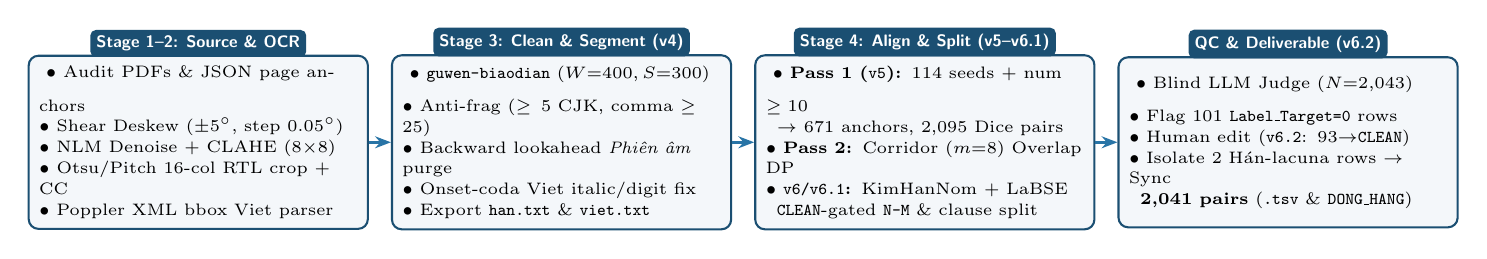
\begin{tikzpicture}[
    node distance=0.28cm,
    stage/.style={rectangle, rounded corners=3.5pt, draw=primary, line width=0.75pt, fill=softbg, text width=4.04cm, minimum height=2.16cm, align=left, font=\scriptsize, inner sep=3.8pt},
    titlebox/.style={rectangle, rounded corners=2pt, fill=primary, text=white, font=\scriptsize\bfseries\sffamily, inner sep=2.2pt},
    arr/.style={-{Stealth[length=2.0mm, width=1.5mm]}, line width=1.05pt, color=secondary}
]
  \node[stage] (s1) {
    \vspace{4.5pt}
    $\bullet$ Audit PDFs \& JSON page anchors\\
    $\bullet$ Shear Deskew ($\pm 5^\circ$, step $0.05^\circ$)\\
    $\bullet$ NLM Denoise + CLAHE ($8{\times}8$)\\
    $\bullet$ Otsu/Pitch 16-col RTL crop + CC\\
    $\bullet$ Poppler XML bbox Viet parser
  };
  \node[titlebox, anchor=south] at ([yshift=-1pt]s1.north) {Stage 1--2: Source \& OCR};

  \node[stage, right=of s1] (s2) {
    \vspace{4.5pt}
    $\bullet$ \texttt{guwen-biaodian} ($W{=}400, S{=}300$)\\
    $\bullet$ Anti-frag ($\ge 5$ CJK, comma $\ge 25$)\\
    $\bullet$ Backward lookahead \textit{Phiên âm} purge\\
    $\bullet$ Onset-coda Viet italic/digit fix\\
    $\bullet$ Export \texttt{han.txt} \& \texttt{viet.txt}
  };
  \node[titlebox, anchor=south] at ([yshift=-1pt]s2.north) {Stage 3: Clean \& Segment (v4)};

  \node[stage, right=of s2] (s3) {
    \vspace{4.5pt}
    $\bullet$ \textbf{Pass 1 (\texttt{v5}):} 114 seeds + num $\ge 10$\\
    \hspace*{4pt}$\to$ 671 anchors, 2,095 Dice pairs\\
    $\bullet$ \textbf{Pass 2:} Corridor ($m{=}8$) Overlap DP\\
    $\bullet$ \textbf{\texttt{v6/v6.1}:} KimHanNom + LaBSE\\
    \hspace*{4pt}\texttt{CLEAN}-gated \texttt{N-M} \& clause split
  };
  \node[titlebox, anchor=south] at ([yshift=-1pt]s3.north) {Stage 4: Align \& Split (v5--v6.1)};

  \node[stage, right=of s3] (s4) {
    \vspace{4.5pt}
    $\bullet$ Blind LLM Judge ($N{=}2{,}043$)\\
    $\bullet$ Flag 101 \texttt{Label\_Target=0} rows\\
    $\bullet$ Human edit (\texttt{v6.2}: 93$\to$\texttt{CLEAN})\\
    $\bullet$ Isolate 2 Hán-lacuna rows $\to$ Sync\\
    \hspace*{4pt}\textbf{2,041 pairs} (\texttt{.tsv} \& \texttt{DONG\_HANG})
  };
  \node[titlebox, anchor=south] at ([yshift=-1pt]s4.north) {QC \& Deliverable (v6.2)};

  \draw[arr] (s1.east) -- (s2.west);
  \draw[arr] (s2.east) -- (s3.west);
  \draw[arr] (s3.east) -- (s4.west);
\end{tikzpicture}
\caption{End-to-end 4-stage code architecture from raw manuscript scans to the finalized 2,041-pair parallel deliverable (\texttt{v6.2}).}
\label{fig:pipeline}
\end{figure}

\vspace{-3pt}
\begin{enumerate}
  \item \textbf{Stage 1--2: Geometry-Aware OCR \& Coordinate Layout Parsing (\texttt{HAN\_OCR\_full.ipynb}, \texttt{viet\_ocr\_batch.py}):}
  \begin{itemize}
    \item \textit{Classical Chinese Auto-Deskewing \& RTL Slicing:} Pages rendered via \texttt{PyMuPDF} crop the bottom 3\% margin (\texttt{CROP\_HEIGHT\_RATIO = 0.97}) to drop scanner artifacts. In \texttt{detect\_auto\_rotation()}, \texttt{spine\_angle()} applies Canny + \texttt{HoughLinesP} on the central gutter ($x\in[0.40W, 0.60W]$) to seed a coarse-to-fine horizontal shear search ($\theta \in [-5^\circ, +5^\circ]$, coarse $0.25^\circ$, fine $0.05^\circ$) over left/right text masks stripped of outer frame strokes via \texttt{connectedComponentsWithStats} ($h_c>0.45H$ or $w_c>0.75W$), maximizing normalized vertical projection variance $J(\theta)=\mathrm{Var}(p_\theta)/(\mu_{p_\theta}^2+10^{-8})$ (e.g., rotating \texttt{Cap\_01} p.\,48 by $-1.20^\circ$ boosts $J$ by $+26.5\%$). After Non-Local Means denoising ($h{=}10$) and \texttt{CLAHE} (\texttt{clipLimit=2.0}, $8{\times}8$ grid), \texttt{detect\_column\_ranges()} computes Otsu vertical projections smoothed by a size-9 median filter, masks the central spine ($\pm 20\text{\,px}$) in \texttt{Cap\_01}, splits merged wide columns ($w>150\text{\,px}$) at local projection minima, and interpolates median column pitch in \texttt{Cap\_02}. \texttt{choose\_border\_columns()} scores edge crops (\texttt{BORDER\_MIN\_SCORE = 2.4}) to prune frame borders without losing any of the 16 RTL columns/page, feeding each padded crop (\texttt{pad=25\,px}) into \textbf{PaddleOCR} (\texttt{chinese\_cht}) while recording polygon $y$-coordinates and per-line confidence.
    \item \textit{Vietnamese XML Bounding-Box \& Anchor Mapping:} \texttt{viet\_ocr\_batch.py} invokes \texttt{pdftotext -bbox-layout}, sorting lines by $(\operatorname{round}(y,1), x)$ and computing page median font height $s_{\text{typ}}$. Lines at $y>0.87H$ matching printed page numbers become \texttt{so\_trang}; bottom regions ($y>0.65H$) with font size $<0.86\,s_{\text{typ}}$ or vertical gap $>1.65\,s_{\text{typ}}$ trigger a sticky footnote state (\texttt{chu\_thich}) that never breaks cross-page prose buffers (\texttt{vắt trang}); regexes on normalized keys switch state machines between \texttt{phien\_am}, \texttt{dich\_tho}, and \texttt{van\_xuoi}. Concurrently, \texttt{page\_mapping()} combines verified cues from \texttt{viet\_han\_anchors.json} with automatic multi-number ($\ge 1{,}000$) page matching.
  \end{itemize}

  \item \textbf{Stage 3: Sliding-Window Classical Punctuation \& Structural \textit{Phiên-Âm} Purge (\texttt{build\_clean\_v3.py}, \texttt{build\_clean\_v4.py}):}
  \begin{itemize}
    \item \textit{Classical Chinese Stream Punctuation:} After dropping duplicate page \texttt{Cap\_01} p.\,49, non-content covers (\texttt{Cap\_02} pp.\,88--92), and running headers (\texttt{撫邊雜錄卷之五/六}), \texttt{punctuate\_char\_stream()} feeds continuous character streams into \texttt{guwen-biaodian} using overlapping sliding windows (\texttt{window\_size=400}, \texttt{stride=300}, keeping inner predictions $[50..350)$ to eliminate boundary truncation effects). \texttt{build\_han\_sentences()} enforces a two-tier anti-fragmentation state machine: terminal marks (\texttt{。！？；}) are downgraded to \texttt{，} if length $<5$ CJK chars (\texttt{MIN\_HAN\_CJK\_CHARS = 5}), long enumerations split at commas once $\ge 25$ chars (\texttt{HAN\_COMMA\_SPLIT\_LEN = 25}), and trailing $<5$-char stubs merge backward, yielding \textbf{2,804 Traditional Chinese sentences} (\texttt{han.txt}, \texttt{le\_4\_chars\_count = 0}) alongside OpenCC \texttt{t2s} embeddings and \texttt{ocr\_conf\_min}.
    \item \textit{100\% Structural \textit{Phiên-Âm} Elimination \& Syllabic Viet Restoration (\texttt{v4}):} Because \texttt{v3}'s \texttt{while}-loop stopped early on keyword-sparse verse (leaving 235 phonetic lines in \texttt{Cap\_02\_V}), \texttt{build\_clean\_v4.py} (\texttt{filter\_cap02\_v\_phien\_am\_structural}) first recovers 5 misclassified bottom-of-page prose sentences (pp.\,32, 95, 97), then scans every interval $(\text{\texttt{prev\_dich\_idx}}, \text{\texttt{d\_idx}})$ upward with a \textbf{2-line upward lookahead} comparing \texttt{ALL\_SV\_MARKERS} ($\ge 0.30$) against \texttt{STRICT\_NATIVE\_VIET} ($\le 0.14$), while \texttt{split\_intro\_from\_phien\_am()} detaches prose lead-ins (\textit{``Đan Bỉnh Ngự hoạ:''}) from attached phonetic verse---purging \textbf{235 leaked \textit{Phiên âm} rows} and trimming \textbf{26 hybrid intros}. Next, \texttt{deterministic\_viet\_clean()} fixes italic OCR \texttt{u}$\to$\texttt{v} confusions (\texttt{uiệc}$\to$\textit{việc}, \texttt{uề}$\to$\textit{về}) via \texttt{ITALIC\_U\_TO\_V\_RHYMES} guarded by \texttt{VALID\_U\_INITIAL\_WORDS}, restores tax digits (\texttt{õ/ð/ã}$\to$\texttt{5}, \texttt{I/l}$\to$\texttt{1} before \textit{quan, tiền, thưng, cáp}), and passes tokens failing Vietnamese onset--nucleus--coda phonotactics (\texttt{is\_suspicious\_viet\_token()}) through a length-guarded ($\pm 20\%$ words) zero-paraphrase typo fixer (\textbf{123 sentences} fixed), outputting \textbf{2,793 pure translation sentences} (\texttt{viet.txt}).
  \end{itemize}

  \item \textbf{Stage 4: Two-Pass Moore-Anchor Overlap DP, Ensemble Splitting \& Human Polish (\texttt{run\_align\_v5.py} $\to$ \texttt{v6.2}):}
  \begin{itemize}
    \item \textit{Pass 1 (Moore/Hunalign Anchor Extraction \& Lexicon Induction) \& Pass 2 (Overlap DP) in \texttt{v5}:} \texttt{PrecomputedCorpusFeatures} pre-indexes Arabic/Hán numeric sets (converting \texttt{一萬四千三百四十九} and \textit{``1 vạn 4349''} identically to \texttt{14349}), \textbf{114 domain seed regexes} (official titles, Thuận--Quảng toponyms, units, \textit{Can Chi} years), and 9 classical discourse boundary particles (\texttt{又}/\textit{Lại}, \texttt{凡}/\textit{Phàm}, \texttt{耳}/\textit{thôi}) for $\mathcal{O}(1)$ bitset union during DP. Pass~1 solves a diagonal band DP ($W\ge 220$) combining \texttt{LaBSE} top-8 cosine similarity with $0.55\,\text{score}_{\text{lex/num}}$ and rare exact numbers ($\ge 20$), extracting \textbf{671 high-confidence \texttt{1-1} anchors} (\texttt{score $\ge 0.58$}). From these anchors, \texttt{induce\_moore\_bilingual\_lexicon()} computes Dice association $\text{Dice}(z,v)=\frac{2c(z,v)}{c(z)+c(v)}$ ($\text{cooc}\ge 3$, $\text{Dice}\ge 0.42$) over CJK 1--2 grams and Viet 1--2 tokens to auto-learn \textbf{2,095 corpus-specific lexical pairs} (capturing OCR-corrupted boat/timber names). Pass~2 locks an anchor-guided corridor (\texttt{win\_margin=8}) and runs multi-overlap DP ($1\le a_1,a_2\le 5$, $a_1{+}a_2\le 7$) using prefix-sum L2-normalized \texttt{LaBSE} vectors with CSLS margin, step-size fairness weighting $1+0.14(a_1{+}a_2-2)$, and \texttt{controlled\_boundary\_smoothing()} (S1 orphan absorption, S2 1-clause boundary shift on \texttt{hybrid\_pair\_cost}, S3 anti-fragmentation merge).
    \item \textit{Ensemble Fine-Splitting (\texttt{v6}), Selective Rollback (\texttt{v6.1}) \& Human Sync (\texttt{v6.2}):} Because \texttt{v5}'s smoothing yields 1,732 pairs ($<2{,}000$), \texttt{run\_refine\_v6\_deliverables.py} reconstructs exact sentence-index beads, repairs 5 local mismatch windows, and partitions \texttt{N-M} clusters via \texttt{local\_dp\_fine\_split()} combining \textbf{KimHanNom API} scores + \texttt{LaBSE} + numeric evidence (238 \texttt{N-M} splits + 37 indexed clause splits $\to$ 2,007 pairs). Observing that splitting noisy boat-roster pages (\texttt{Cap\_01} pp.\,33--40, where \texttt{銃} misreads as \texttt{說/視}) inflated \texttt{PARTIAL} labels, \texttt{run\_refine\_v6\_1.py} \textbf{rolls back every \texttt{v6} split whose sub-pairs were not 100\% \texttt{CLEAN}} under blind evaluation, freezes \texttt{Cap\_01} pp.\,33--40, and applies lossless \texttt{IndexedSplitDecision} strictly on high-OCR ($\ge 0.65$) compound clauses (\textbf{2,037 pairs}). Finally, in \textbf{\texttt{v6.2}}, all 101 flagged rows (\texttt{DANH\_SACH\_DONG\_CAN\_RA\_SOAT\_V6\_1.md}) undergo manual boundary editing in Excel, and \texttt{sync\_and\_judge\_final\_deliverable.py} isolates 2 archival Hán-lacuna rows to export \textbf{2,041 identical valid pairs} to \texttt{.tsv} and \texttt{DONG\_HANG}.
  \end{itemize}
\end{enumerate}

\begin{figure}[!htb]
\centering
\begin{tabular}{@{}c@{\hspace{5pt}}c@{\hspace{5pt}}c@{\hspace{7pt}}m{5.25cm}@{}}
  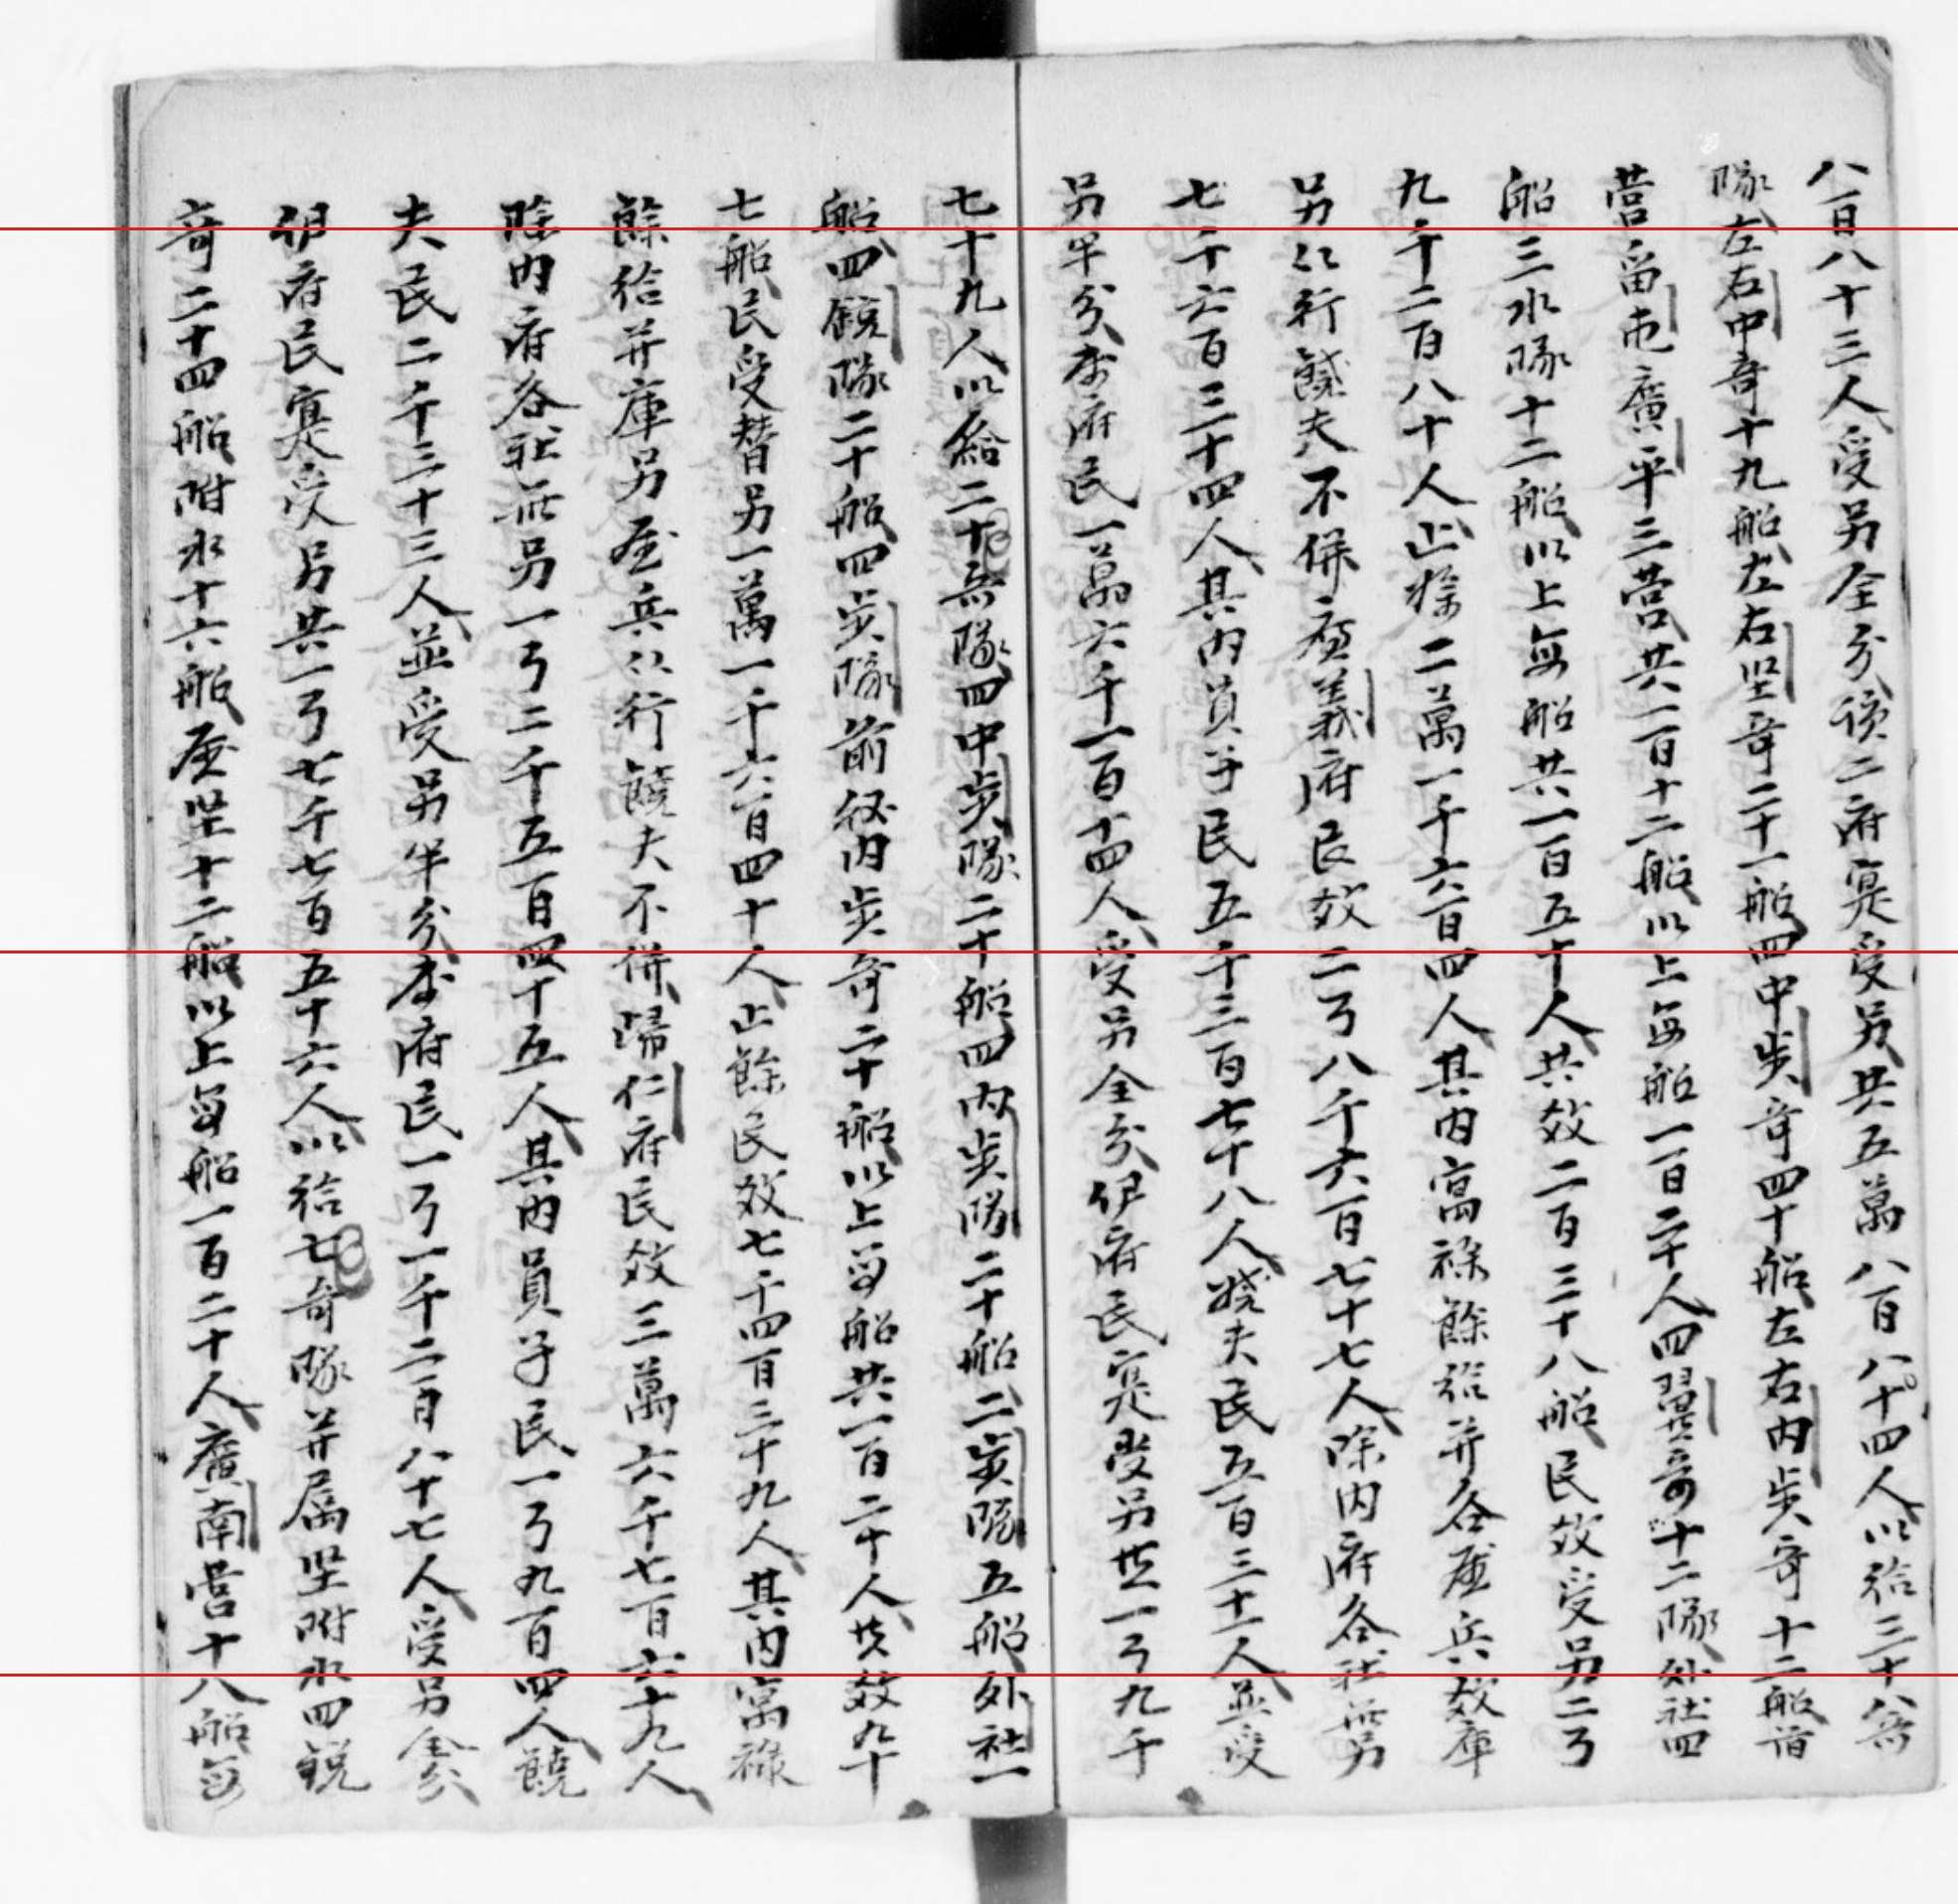
\includegraphics[height=3.65cm]{figures/cap01_p48_raw_skewed.jpg} &
  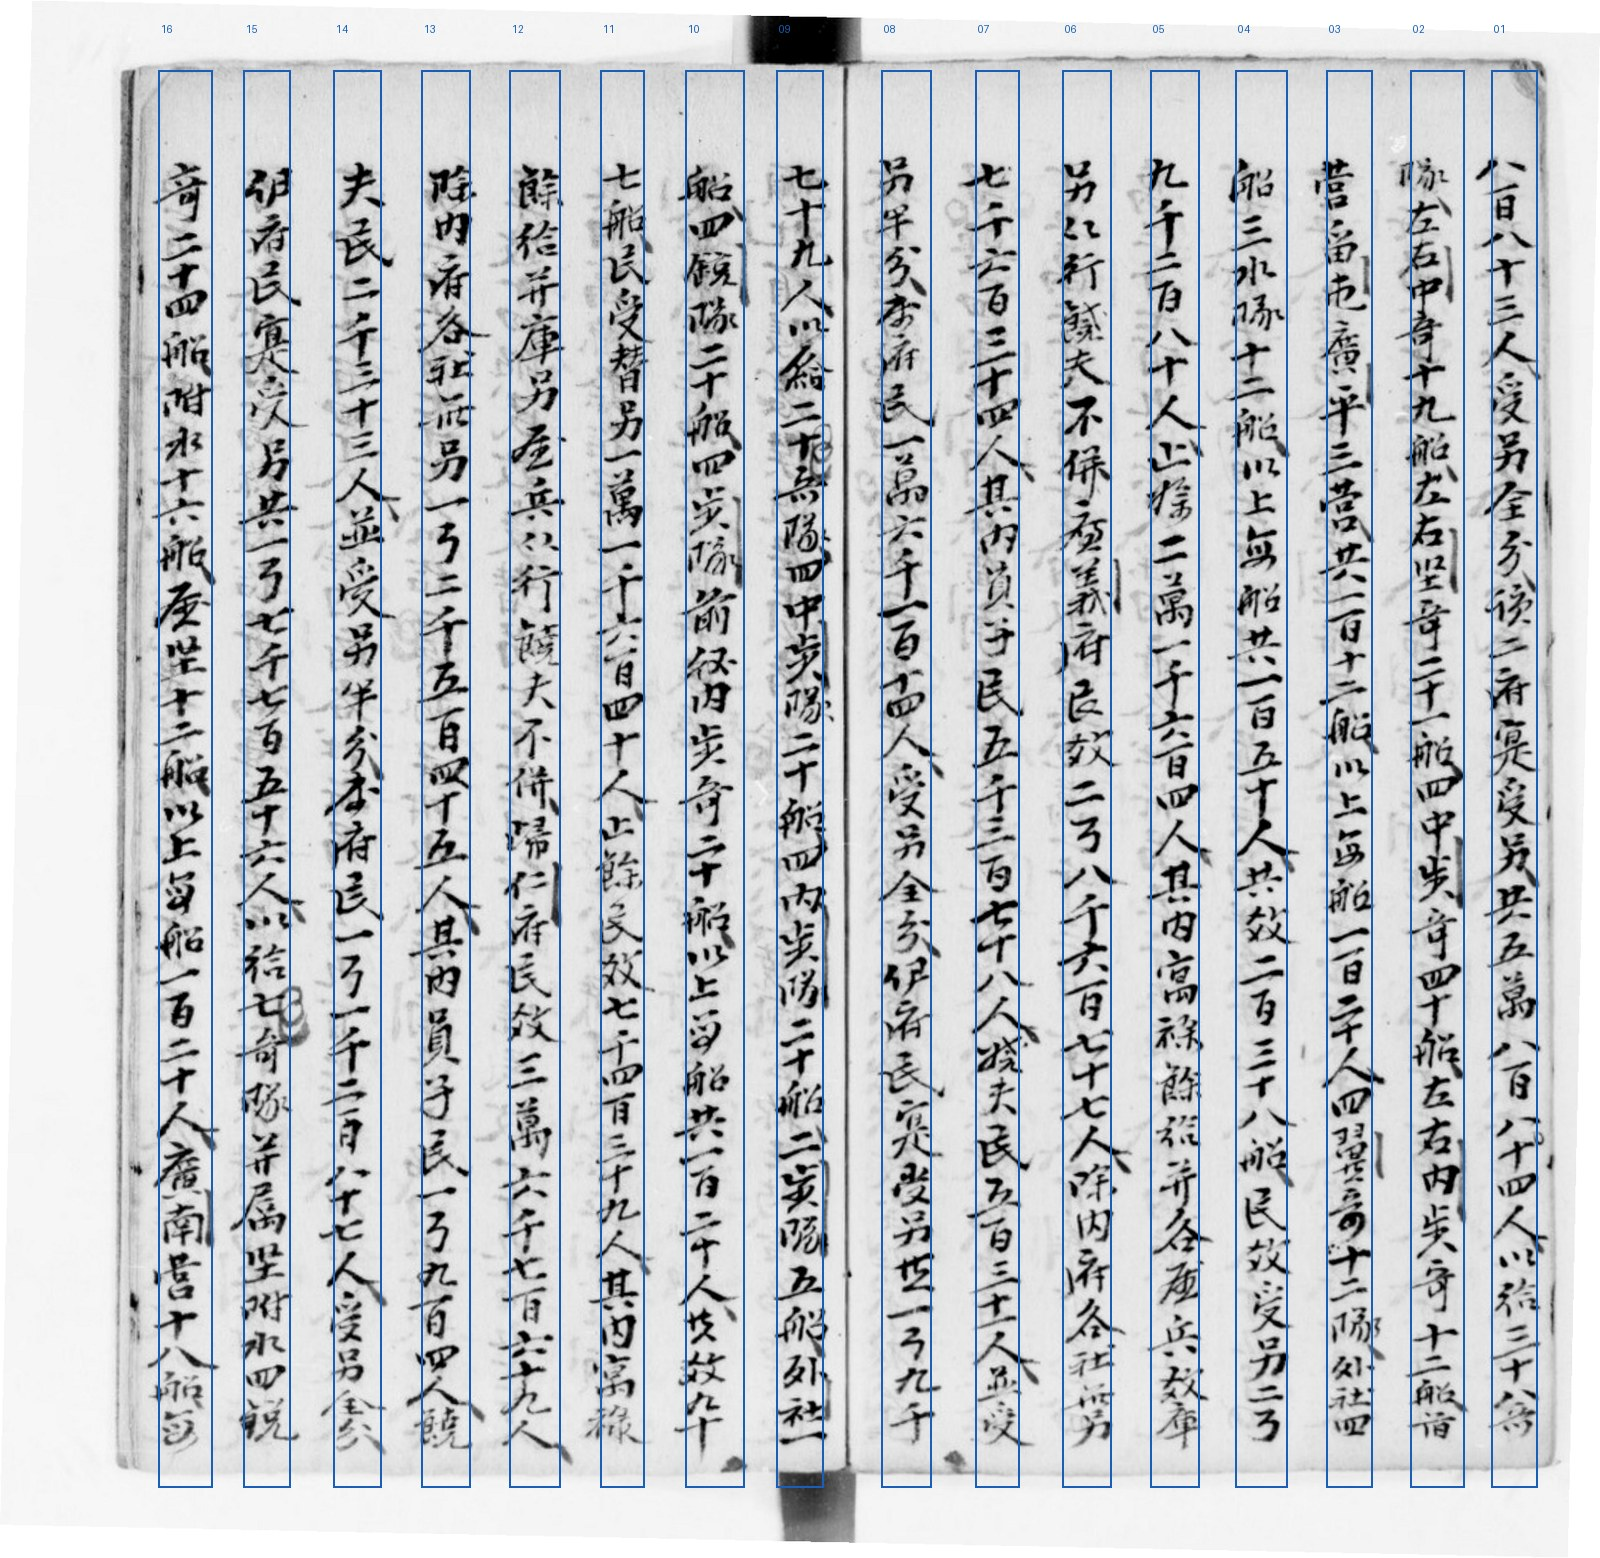
\includegraphics[height=3.65cm]{figures/cap01_p48_deskew_cols.jpg} &
  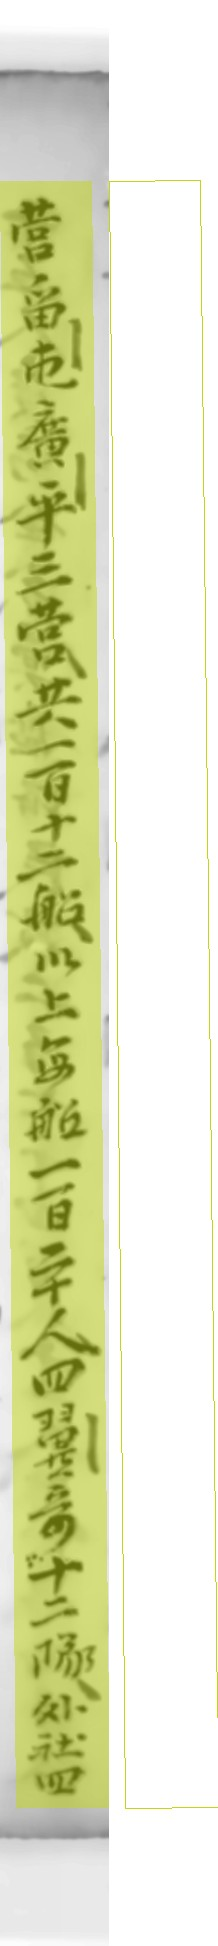
\includegraphics[height=3.65cm]{figures/paddleocr_col_p48.jpg} &
  \vspace{-3.55cm}\fcolorbox{bordercol}{softbg}{%
    \parbox{5.00cm}{\scriptsize\raggedright
      \textbf{\textcolor{primary}{(d) Code Trace Col.\,03 $\to$ \texttt{P0729\_C048\_V246}:}}\\[1.5pt]
      \textbf{1. PaddleOCR} (\texttt{conf=0.81}, $-1.20^\circ$ deskew):\\
      營留屯廣平三營共一百十二般川上每船一百二十人四奇十二陽外四\\[1.5pt]
      \textbf{2. \texttt{guwen-biaodian} + \texttt{PrecomputedFeatures}:}\\
      Nums $\{112, 120, 4, 12\}$ + Seeds \texttt{營,船}$\leftrightarrow$\textit{dinh, thuyền}\\[1.5pt]
      \textbf{3. Final Synced Output (\texttt{1-2}, \texttt{CLEAN}):}\\
      \textbf{ZH:} 共一百十二般，川上每船一百二十人，四奇十二，陽外四船三，水隊十二船。\\[1pt]
      \textbf{VI:} Ba dinh Cựu Dinh, Lưu Đồn, Quảng Bình, cộng \textbf{112} thuyền, mỗi thuyền \textbf{120} người. Bốn dực cơ 19 đội, ngoại xã \textbf{4} thuyền, đội Tam thuỷ \textbf{12} thuyền, mỗi thuyền 150 người.
    }%
  } \\
  {\scriptsize \textbf{(a)} Raw scan (\texttt{Cap\_01} p.\,48, $-1.20^\circ$)} &
  {\scriptsize \textbf{(b)} Deskewed + 16 RTL cols (\texttt{01}--\texttt{16})} &
  {\scriptsize \textbf{(c)} Col.\,03} &
\end{tabular}
\caption{ Step-by-step code trace on \texttt{Cap\_01} Page 48: (a) skewed scan with dark gutter, (b) shear-variance deskewing ($+26.5\%$) and CC border-filtered 16-column RTL slicing, (c) vertical PaddleOCR detection, and (d) numeric/seed-anchored pair \texttt{P0729\_C048\_V246}.}
\label{fig:ocr_visual}
\end{figure}

% ==============================================================================
% 4. ACHIEVED RESULTS
% ==============================================================================
\section{Achieved Results}
\textbf{Final Deliverables \& Corpus Volume:} From 140 Classical Chinese content pages (\textbf{51,791 CJK characters}; \textbf{2,804 sentences} in \texttt{han.txt}) and 206 Vietnamese pages (\textbf{2,793 translation sentences} in \texttt{viet.txt}), the finalized \textbf{Version 6.2} pipeline exports \textbf{2,041 valid parallel pairs} (\texttt{MISSING = 0}) identically across \texttt{CV16\_PhuBienTapLuc\_parallel.tsv} and the \texttt{DONG\_HANG} sheet of \texttt{.xlsx} (Table~\ref{tab:results}). Automated QC passes \textbf{1,886 pairs (92.41\% \texttt{Label\_Target=1})} and \textbf{95.00\% \texttt{OCR\_Valid}} ($\ge 0.55$). Distribution across Guideline alignment types reflects fine clause granularity: \textbf{56.74\% \texttt{1-1}} (1,158), \textbf{20.33\% \texttt{1-2}/\texttt{2-1}} (415), \textbf{7.25\% \texttt{2-2}} (148), and \textbf{15.68\%} multi-clause merges (Table~\ref{tab:examples}).

\begin{table}[!htb]
\centering
\caption{Quantitative summary of cleaned text (\texttt{03/v4}) and final synchronized deliverable (\texttt{04/v6.2}) across corpus blocks.}
\label{tab:results}
\scriptsize
\setlength{\tabcolsep}{3.6pt}
\renewcommand{\arraystretch}{1.08}
\begin{tabularx}{\textwidth}{@{}Y r r r r r c c c c c@{}}
\toprule
\textbf{Corpus Block} & \textbf{Hán} & \textbf{CJK} & \textbf{Việt} & \textbf{Valid Pairs} & \textbf{\texttt{Label=1} (\%)} & \textbf{\texttt{1-1} / \texttt{1-2,2-1}} & \textbf{\texttt{CLEAN} (\%)} & \textbf{\texttt{PARTIAL}} & \textbf{\texttt{MISMATCH}} & \textbf{\texttt{USABLE}} \\
\midrule
\texttt{Cap\_01} (Tax/Military) & 1,145 & 23,261 & 1,172 & 788 & 705 (89.47\%) & 387 / 179 & 556 (70.56\%) & 230 (29.19\%) & \textbf{2 (0.25\%)} & \textbf{99.75\%} \\
\texttt{Cap\_02\_V} (Poetry/Prose) & 982 & 16,973 & 1,059 & 779 & 729 (93.58\%) & 467 / 147 & 670 (86.01\%) & 107 (13.74\%) & \textbf{2 (0.26\%)} & \textbf{99.74\%} \\
\texttt{Cap\_02\_VI} (Geography) & 677 & 11,557 & 562 & 474 & 452 (95.36\%) & 304 / 89 & 371 (78.27\%) & 101 (21.31\%) & \textbf{2 (0.42\%)} & \textbf{99.58\%} \\
\midrule
\textbf{Total (\texttt{v6.2} Final)} & \textbf{2,804} & \textbf{51,791} & \textbf{2,793} & \textbf{2,041} & \textbf{1,886 (92.41\%)} & \textbf{1,158 / 415} & \textbf{1,597 (78.25\%)} & \textbf{438 (21.46\%)} & \textbf{6 (0.29\%)} & \textbf{99.71\%} \\
\bottomrule
\end{tabularx}
\end{table}

\vspace{-3pt}
\begin{table}[!htb]
\centering
\caption{Illustrative aligned pairs across genres from final deliverable \texttt{04\_dong\_hang/CV16\_PhuBienTapLuc\_parallel.xlsx}.}
\label{tab:examples}
\scriptsize
\renewcommand{\arraystretch}{1.08}
\begin{tabularx}{\textwidth}{@{}l c L{5.75cm} Y@{}}
\toprule
\textbf{Pair ID (Block)} & \textbf{Type} & \textbf{Classical Chinese (\texttt{Hán})} & \textbf{Vietnamese Translation (\texttt{Việt})} \\
\midrule
\texttt{P0009\_C001\_V187} (\texttt{Cap\_01}) & \texttt{1-1} & 卯已丑，升華府各縣屬一萬四千三百四十九人，收各歲共四百八十三。 & Như năm Kỷ Sửu các huyện thuộc phủ Thăng Hoa cộng 1 vạn 4349 người, thu các tiền cộng 483 quan 3 tiền 36 đồng, \\
\texttt{P0433\_C028\_V222} (\texttt{Cap\_01}) & \texttt{1-1} & 花綾匠人數二十五人，收花綾綵四十六疋三尺（每疋十尺）。 & Thợ dệt lĩnh hoa, số người 25 người, thu hàng lĩnh hoa 46 tấm 3 thước (mỗi tấm 10 thước). \\
\texttt{P0839\_C004\_V012} (\texttt{Cap\_02\_V}) & \texttt{1-1} & 撐持江漢雙枝櫂， & Vẫy vùng giang hán chèo đôi mái; \\
\texttt{P1702\_C061\_V415} (\texttt{Cap\_02\_VI}) & \texttt{1-1} & 廣南會安庯，銅鍋銅盤，洋船販到，平辰以千萬計。 & Phố Hội An xứ Quảng Nam, nồi đồng mâm đồng, do tàu Tây phương chở đến bán, bình thời kể có hàng nghìn hàng vạn, \\
\bottomrule
\end{tabularx}
\end{table}

% ==============================================================================
% 5. EVALUATION AND DISCUSSION
% ==============================================================================
\needspace{6\baselineskip}
\section{Evaluation and Discussion}
\subsection{Full-Corpus Blind Evaluation and Quality Compliance}
Every version from \texttt{v4} to \texttt{v6.2} is evaluated across \textbf{100\% of corpus rows ($N=2{,}041$)} using a blind independent \textbf{LLM-as-a-Judge} protocol (\texttt{judge\_real\_label.py}, \texttt{gemini-3.5-flash-lite}, \texttt{temperature=0.0}, batch size 20, stripping all prior flags) paired with deterministic heuristic gates under $\text{Error Rate} = N_{\text{error}} / N_{\text{valid}}$ (Figure~\ref{fig:eval_chart}):
\begin{itemize}
  \item \textbf{Guideline Error Rate \& Heuristic Verification:} Across all 2,041 deliverable pairs, \texttt{MISSING = 0\%}, heuristic warnings are tightly bounded (\texttt{OMISSION} 1.71\%, \texttt{ADDITION} 0.59\%, low OCR 5.00\%), and blind semantic auditing confirms \textbf{1,597 \texttt{CLEAN} pairs (78.25\%)}, \textbf{438 \texttt{PARTIAL} pairs (21.46\%)}, and \textbf{only 6 \texttt{MISMATCH} pairs (0.29\%)}. Overall semantic usability reaches \textbf{99.71\% (2,035/2,041)}, while the \textbf{0.29\%} error rate is two orders of magnitude below the \textbf{$\le$ 30\%} Guideline limit ($\le$ 20\% internal safety target).
  \item \textbf{Human-in-the-Loop Gain (\texttt{v6.1} $\to$ \texttt{v6.2}):} Targeted manual editing of 101 flagged boundary rows (Quảng Ngãi/Quy Nhơn silk-weaver tax tables in \texttt{Cap\_01} pp.\,27--29, boat rosters in pp.\,34--36, and \textit{Hà Tiên thập vịnh} verse in \texttt{Cap\_02\_V}) promoted \textbf{93/101 edited rows directly to \texttt{CLEAN}}, cutting \texttt{MISMATCH} errors by \textbf{88.0\%} (50 $\to$ \textbf{6 rows}) and lifting \texttt{Cap\_02\_V} \texttt{CLEAN} rate to \textbf{86.01\%}.
\end{itemize}

\begin{figure}[!htb]
\centering
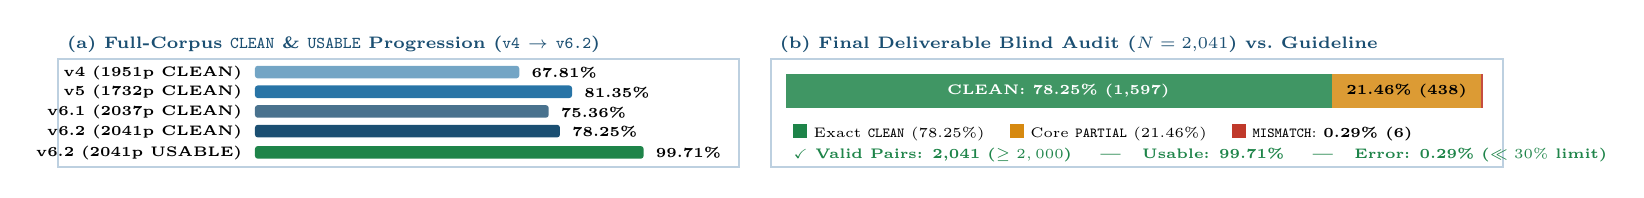
\begin{tikzpicture}[font=\scriptsize]
  \node[anchor=west, font=\scriptsize\bfseries\color{primary}] at (0, 1.56) {(a) Full-Corpus \texttt{CLEAN} \& \texttt{USABLE} Progression (\texttt{v4} $\to$ \texttt{v6.2})};
  \draw[bordercol, thick] (0,0) rectangle (8.65, 1.38);
  \foreach \y/\lbl/\val/\col in {1.11/v4 (1951p CLEAN)/67.81/secondary!65, 0.86/v5 (1732p CLEAN)/81.35/secondary, 0.61/v6.1 (2037p CLEAN)/75.36/primary!80, 0.36/v6.2 (2041p CLEAN)/78.25/primary, 0.09/v6.2 (2041p USABLE)/99.71/okgreen} {
    \node[anchor=east, font=\tiny\bfseries] at (2.45, \y+0.09) {\lbl};
    \fill[\col, rounded corners=1pt] (2.50, \y+0.02) rectangle ({2.50 + \val*0.0495}, \y+0.18);
    \node[anchor=west, font=\tiny\bfseries] at ({2.54 + \val*0.0495}, \y+0.09) {\val\%};
  }

  \node[anchor=west, font=\scriptsize\bfseries\color{primary}] at (9.05, 1.56) {(b) Final Deliverable Blind Audit ($N=2{,}041$) vs.\ Guideline};
  \draw[bordercol, thick] (9.05,0) rectangle (18.35, 1.38);
  \fill[okgreen!85] (9.25, 0.75) rectangle ({9.25 + 8.85*0.7825}, 1.18);
  \fill[warnamber!85] ({9.25 + 8.85*0.7825}, 0.75) rectangle ({9.25 + 8.85*0.9971}, 1.18);
  \fill[accent!90] ({9.25 + 8.85*0.9971}, 0.75) rectangle (18.10, 1.18);
  \node[text=white, font=\tiny\bfseries] at ({9.25 + 8.85*0.39}, 0.965) {CLEAN: 78.25\% (1,597)};
  \node[text=black, font=\tiny\bfseries] at ({9.25 + 8.85*0.89}, 0.965) {21.46\% (438)};
  \node[anchor=west, font=\tiny] at (9.22, 0.44) {\textcolor{okgreen}{\rule{5pt}{5pt}} Exact \texttt{CLEAN} (78.25\%) \quad \textcolor{warnamber}{\rule{5pt}{5pt}} Core \texttt{PARTIAL} (21.46\%) \quad \textcolor{accent}{\rule{5pt}{5pt}} \texttt{MISMATCH}: \textbf{0.29\% (6)}};
  \node[anchor=west, font=\tiny\bfseries\color{okgreen}] at (9.22, 0.16) {$\checkmark$ Valid Pairs: 2,041 ($\ge 2,000$) \quad|\quad Usable: 99.71\% \quad|\quad Error: 0.29\% ($\ll 30\%$ limit)};
\end{tikzpicture}
\caption{Progression across alignment versions (\texttt{v4}$\to$\texttt{v6.2}) and full-corpus blind LLM-as-a-Judge audit on the 2,041-pair deliverable.}
\label{fig:eval_chart}
\end{figure}

\vspace{-3pt}
\subsection{Iterative Bottlenecks and Root-Cause Analysis Across All Versions (\texorpdfstring{\texttt{v2} $\to$ \texttt{v6.2}}{v2 to v6.2})}
\begin{table}[!htb]
\centering
\caption{Complete evolution of mechanisms, full-corpus blind metrics, bottlenecks, and root-cause solutions from \texttt{v2} to \texttt{v6.2}.}
\label{tab:versions}
\scriptsize
\setlength{\tabcolsep}{3.4pt}
\renewcommand{\arraystretch}{1.07}
\begin{tabularx}{\textwidth}{@{}L{1.80cm} L{3.40cm} L{3.35cm} Y@{}}
\toprule
\textbf{Version} & \textbf{Core Mechanism} & \textbf{Key Quantitative Metrics} & \textbf{Encountered Bottleneck \& Root-Cause Analysis} \\
\midrule
\textbf{v2} \newline \textit{(Baseline)} & Full-block Bertalign on basic cleaned text (\texttt{COMMA\_LEN=15}). & \textbf{2,451} pairs (2,415 valid); \texttt{Label=1}: 92.49\%; Strict \texttt{real\_label} $\sim$\textbf{55.0\%}. & \textbf{Issue/Cause:} Unfiltered Sino-Vietnamese \textit{Phiên âm} before \texttt{(Dịch):} locally doubled Viet sentence counts, causing cascading drift in \texttt{Cap\_02\_V}; loose cap (\texttt{4.50}) hid merges. \\
\addlinespace[1.1pt]
\textbf{v3} \newline \textit{(Hard Window)} & \texttt{03/v3} initial \textit{Phiên âm} filter + hard 5-page Hán window slicing. & \textbf{2,174} pairs; \texttt{MISSING} spiked to \textbf{293} (13.48\%); \texttt{Anchor} 27.32\%. & \textbf{Issue/Cause:} Hard-cutting Viet index \texttt{v\_cut} at 5-page boundaries stranded cross-window counterparts (206 \texttt{0-1}, 87 \texttt{1-0}); $|\#_{\text{zh}}-\#_{\text{vi}}|\le 2$ over-penalized tax tables. \\
\addlinespace[1.1pt]
\textbf{v3.1} \newline \textit{(3-Phase Shift)} & Full-block Bertalign (\texttt{max\_align=5}) + 3-phase boundary shift. & \textbf{1,938} pairs; \texttt{MISSING} cut by \textbf{90\%} ($\to$29); Strict clean $\to$\textbf{73.6\%}. & \textbf{Issue/Cause:} \texttt{Cap\_01} lagged at \textbf{53.3\%} (208 numeric flags) because \texttt{LaBSE} failed to match Hán numerals (\texttt{四千八百廿}) with Arabic digits (\texttt{4820}) in repetitive formulas. \\
\addlinespace[1.1pt]
\textbf{v4} \newline \textit{(Numeric-Norm)} & Hán$\to$Arabic internal norm + value ($\ge 10$) \& particle shift. & \textbf{1,951} pairs (1,923 valid); Blind Judge: \texttt{CLEAN} \textbf{67.81\%}, Err \textbf{6.71\%}. & \textbf{Issue/Cause:} Below 2,000 pairs; 131 \texttt{MISMATCH} rows (72 in \texttt{02\_V}) because \texttt{03/v3}'s \texttt{while}-loop halted early on sparse verse, leaving \textbf{235 leaked \textit{Phiên âm} rows}. \\
\addlinespace[1.1pt]
\textbf{v5} \newline \textit{(Moore 2-Pass)} & \texttt{03/v4} 100\% \textit{Phiên âm} purge + 671 Moore anchors + 2,095 Dice pairs + Overlap smoothing. & \textbf{1,732} pairs (1,730 valid); \texttt{CLEAN} \textbf{81.35\%} (1,409); Err \textbf{1.96\%}; \texttt{USABLE} \textbf{98.04\%}. & \textbf{Issue/Cause:} Peak autonomous accuracy (81.35\% \texttt{CLEAN}), but anti-fragmentation smoothing merged comma-linked clauses into 480 \texttt{N-M} clusters, dropping below 2,000 pairs. \\
\addlinespace[1.1pt]
\textbf{v6} \newline \textit{(Ensemble Split)} & \texttt{v5} + \textbf{KimHanNom API} + LaBSE DP splitting 238 \texttt{N-M} \& 37 clauses. & \textbf{2,008} pairs (\textbf{2,007} valid); Err \textbf{0.80\%} (16), \texttt{USABLE} \textbf{99.20\%}; \texttt{CLEAN} \textbf{68.18\%}. & \textbf{Issue/Cause:} Surpassed 2,000 pairs with 0.80\% error, but splitting inside low-OCR boat rosters (\texttt{Cap\_01} pp.\,33--40, \texttt{銃}$\to$\texttt{說/視}) exposed 1-clause slips (\texttt{PARTIAL} 31.03\%). \\
\addlinespace[1.1pt]
\textbf{v6.1 $\to$ v6.2} \newline \textit{(Selective + Human)} & \texttt{v6.1}: Rollback non-\texttt{CLEAN} splits + high-OCR clause split; \texttt{v6.2}: Manual edit 101 rows + sync. & \texttt{v6.1}: 2,037p (\texttt{CLEAN} 75.36\%)$\to$\textbf{\texttt{v6.2}: 2,041 valid; \texttt{CLEAN} 78.25\%; Err 0.29\% (6); \texttt{USABLE} 99.71\%}. & \textbf{Resolution:} \texttt{v6.1} recovered +7.18\%p \texttt{CLEAN} via \texttt{CLEAN}-gated rollback; \texttt{v6.2} manual polish converted 93/101 flagged rows to \texttt{CLEAN} and isolated 2 source-lacuna rows. \\
\bottomrule
\end{tabularx}
\end{table}

% ==============================================================================
% 6. IN-DEPTH CONCLUSION, ERROR TAXONOMY, AND FUTURE WORK
% ==============================================================================
\needspace{10\baselineskip}
\section{Conclusion, Fine-Grained Error Analysis, and Future Work}
\subsection{Summary of Engineering and Corpus Contributions}
\begin{itemize}
  \item \textbf{Domain-Specialized Historical NLP Pipeline:} Designed a deterministic-first, fully traceable codebase overcoming three core bottlenecks of Sino-Vietnamese historical scans: (i) shear-variance auto-deskewing and CC-filtered 16-column RTL slicing (\texttt{02\_ocr\_tho}); (ii) 2-line upward-lookahead \textit{Phiên âm} elimination (removing all 235 leaked phonetic verse lines) paired with syllabic onset--coda Vietnamese OCR restoration and overlap-window \texttt{guwen-biaodian} segmentation (\texttt{03/v4}: 2,804 Hán / 2,793 Việt sentences); and (iii) a \textbf{Two-Pass Moore/Hunalign Lexical-Numeric Anchor + Vecalign Overlap Aligner (\texttt{v5})} coupled with \textbf{KimHanNom API} \texttt{CLEAN}-gated splitting (\texttt{v6.1}).
  \item \textbf{High-Precision Deliverable Corpus (\texttt{CV16\_PhuBienTapLuc}):} Delivered \textbf{2,041 valid aligned pairs} (\texttt{MISSING = 0}, 100\% line-by-line parity between \texttt{.tsv} and Excel \texttt{DONG\_HANG}), achieving \textbf{78.25\% strict \texttt{CLEAN}} (1,597), \textbf{99.71\% \texttt{USABLE}} (2,035), \textbf{92.41\% \texttt{Label\_Target=1}}, and a \textbf{0.29\% alignment error rate} ($\ll$ 20\% internal \& 30\% Guideline thresholds) under 100\% full-corpus blind auditing.
\end{itemize}

\subsection{Root-Cause Taxonomy of Remaining Imperfections and Limitations}
A granular code-and-data inspection of all non-\texttt{CLEAN} outputs in \texttt{v6.2} reveals four structural limitations of historical OCR alignment:
\begin{enumerate}
  \item \textbf{Micro-Analysis of the Only 6 Remaining \texttt{MISMATCH} Pairs (\texttt{0.29\%}) \& 2 Archival Lacunae:}
  (a) \textit{Adjacent header/clause inversion around heavily corrupted calligraphy} (\texttt{P0157}--\texttt{P0158} on \texttt{Cap\_01} p.\,10/V199, where cursive \texttt{例}/\texttt{赦} misread as \texttt{疾到}/\texttt{陣除}, and diplomatic letter \texttt{P0963} on \texttt{Cap\_02\_V} p.\,12/V28);
  (b) \textit{Untranslated source verse} (\texttt{P1440}, p.\,42/V90: the published 2007 Vietnamese edition itself prints only Sino-Vietnamese \textit{Phiên âm} \textit{``Nhất thiên khai thự sắc...''} without a vernacular \textit{(Dịch)} poem);
  (c) \textit{Severe stroke coalescence in cursive medical/textile notes} (\texttt{P1785} \textit{kỳ nam/trầm hương} p.\,67/V421 and \texttt{P1833} p.\,71/V424, where \texttt{織布} degraded into \texttt{不識}); and
  (d) \textit{Cross-edition lacunae:} Two boat-roster entries on Viet p.\,233 (\textit{đội Hậu bính}, 4 boats / 225 men) are absent in the Gallica BnF \textit{Vietnamien A 18} manuscript and were properly isolated from \texttt{DONG\_HANG} to preserve strict bilingual validity.
  \item \textbf{Anatomy of the 438 \texttt{PARTIAL} Pairs (\texttt{21.46\%}) \& Punctuation Asymmetry:}
  Nearly half of \texttt{PARTIAL} rows (\texttt{212/438 = 48.4\%}) are \texttt{1-1} pairs and \texttt{95.7\%} (419/438) already have \texttt{OCR\_Valid = 1}. Their \texttt{PARTIAL} status stems not from misalignment, but from \textit{structural punctuation divergence}: \texttt{guwen-biaodian} places periods inside continuous Classical Chinese tax/boat ledgers (\texttt{Cap\_01} accounts for 230/438 \texttt{PARTIAL} rows, e.g., \textit{``...thu tiền X quan, gạo Y bao...''}) at slightly different clause breaks than the modern Vietnamese translator's semicolons, leaving a minor trailing phrase attached across neighbor pairs while 100\% of core figures and entities match.
  \item \textbf{Resilience vs.\ Fragility Under Cursive OCR Noise (\texttt{OCR\_Conf\_Min < 0.55}):}
  Among the 102 low-confidence Hán rows (\texttt{5.00\%}), our numeric/Moore-lexicon anchors still aligned \textbf{83/102 (81.37\%) as \texttt{CLEAN}} and \textbf{19/102 (18.63\%) as \texttt{PARTIAL}} (\textbf{0\% \texttt{MISMATCH}}). Nevertheless, glyph substitutions on rare boat names (\texttt{銃}$\to$\texttt{說/視/鏡}) cap fine-splitting granularity in \texttt{Cap\_01} pp.\,33--40 and degrade downstream lexical lookup if left uncorrected at character level.
  \item \textbf{Pre-trained Embedding Domain Gap (\textit{Wenyan} vs.\ \textit{Baihua}):}
  \texttt{LaBSE} is trained predominantly on Modern Chinese; on allusions, parallel prose (\textit{biền văn}), and inverted Tang couplets in \texttt{Cap\_02\_V}, raw cosine margins flatten ($<0.15$), making our two-pass lexical-numeric anchor corridor and \texttt{CLEAN}-gated verification indispensable but computationally heavier than single-pass bi-encoder retrieval.
\end{enumerate}

\subsection{Concrete Future Directions and Technical Roadmap}
\begin{enumerate}
  \item \textbf{Confidence-Guided Character-Level Hán OCR Post-Correction:} Crop original column polygons in \texttt{02\_ocr\_tho/} (\texttt{Cap\_01/HAN/raw/}) for the 102 \texttt{OCR\_Conf\_Min < 0.55} rows and the 5 OCR-induced \texttt{MISMATCH} pairs, combining a Multimodal VLM (\texttt{Gemini} Vision) with Classical Chinese language-model constraints constrained by the verified Vietnamese translation (e.g., restoring \texttt{說/視}$\to$\texttt{銃} when aligned with \textit{thuyền ... súng}) without hallucinating unattested characters.
  \item \textbf{Joint Bilingual Clause Re-segmentation for \texttt{PARTIAL} Tax Ledgers:} Replace static pre-alignment punctuation in continuous \texttt{Cap\_01} enumerations with joint bilingual clause boundary projection, dynamically re-placing \texttt{。}/semicolon breaks at recurring ledger syntactic triggers (\texttt{收錢}/\textit{thu tiền}, \texttt{除給}/\textit{trừ cấp}, \texttt{存納稅}/\textit{còn nộp thuế}) to convert $>300$ \texttt{PARTIAL} rows into strict \texttt{1-1 CLEAN} pairs.
  \item \textbf{Domain-Adapted Classical Sino-Vietnamese Bi-Encoder \& Full-Book Scaling:} Fine-tune \texttt{OmniAlign} / \texttt{BGE-M3} via contrastive InfoNCE loss using our 1,597 verified \texttt{CLEAN} pairs as positives and adjacent same-page tax/verse rows as hard negatives, then deploy the fine-tuned aligner across Volumes I--III of \textit{Phủ Biên Tạp Lục} and related 18th-century Sino-Vietnamese gazetteers (\textit{Đại Nam nhất thống chí}, \textit{Lịch triều hiến chương loại chí}).
\end{enumerate}

\end{document}
